\documentclass[10pt]{article}

\usepackage{times,fullpage,graphicx,amsmath, subfigure}
\usepackage[pdfborder={0 0 0}]{hyperref}

\title{The Smithlab DNA Methylation Data Analysis Pipeline (MethPipe)} 
\author{Qiang Song \and Michael Kessler \and Fang Fang \and
  Jenny Qu \and Tyler Garvin \and Meng Zhou \and Ben Decato \and Andrew Smith}

\newcommand{\meth}{\texttt{methpipe}}

%%%%
%%%% NOTE: use the following appropriately so that we can change the
%%%% individual types later.
%%%%
%%
%% For program names
\newcommand{\prog}[1]{\texttt{#1}}
%% For file names
\newcommand{\fn}[1]{\texttt{#1}}
%% For literals
\newcommand{\lit}[1]{\texttt{#1}}
%% For program options
\newcommand{\op}[1]{\texttt{#1}}

\begin{document}

\maketitle

The \meth{} software package is a comprehensive pipeline and set of
tools for analyzing whole genome bisulfite sequencing data
(BS-seq). This manual explains the stages in our pipeline, how to use
the analysis tools, and how to modify the pipeline for your specific
context.

\section{Assumptions}

Our pipeline was designed to run in a cluster computing context, with
many processing nodes available, and a job submission system like PBS
or SGE. Much of this analysis is computationally intensive. We assume
that individual nodes will have several GB of memory available for
processing. Typically the data we deal with amounts to a minimum of
100GB for a mammalian methylome at 10x coverage. Intermediate files
may cause this amount to more than double during execution of the
pipeline, and likely at the end of the pipeline the total size of
files will amount to almost double the size of the raw data.

Users are assumed to be quite familiar with UNIX/Linux and related
concepts ({\em e.g.} building software from source, using the command
line, shell environment variables, etc.).

It is also critical that users are familiar with BS-seq experiments,
especially the bisulfite conversion reaction, and how this affects
what we observe in the sequenced reads. Especially if paired-end
sequencing is used. If you do not understand these concepts, you will
likely run into major problems trying to customize our pipeline.

\section{Methylome construction}

\subsection{Mapping reads}
\label{sec:mapping}

% \begin{description}
% \item[rmapbs.cpp]
% This program takes fastq file as input and output mapped read file
% \end{description}

During bisulfite treatment, unmethylated cytosines in the original DNA
sequences are converted to uracils, which are then incorporated as
thymines (T) during PCR amplification. These PCR products are referred
to as T-rich sequences as a result of their high thymine
constitution. With paired-end sequencing experiments, the compliments
of these T-rich sequences are also sequenced.  These complimentary
sequences have high adenosine (A) constitution (A is the complimentary
base pair of T), and are referred to as A-rich sequences. Mapping
consists of finding sequence similarity, based on context specific
criteria, between these short sequences, or reads, and an orthologous
reference genome.  When mapping T-rich reads to the
reference genome, either a cytosine (C) or a thymine (T) in a read is
considered a valid match for a cytosine in the reference genome. For
A-rich reads, an adenine or a guanine is considered a valid match for
a guanine in the reference genome. The mapping of reads to the
reference genome by \prog{rmapbs} is described below. If you choose
to map reads with a different tool, make sure that your post-mapping
files are appropriately formatted for the next components of the
\meth{} pipeline (necessary file formats for each step are covered in
the corresponding sections).  The default behavior of rmapbs is to
assume that reads are T-rich and map accordingly. To change the
mapping to suit A-rich reads, add the \op{-A} option.

\paragraph{Input and output file formats:} We assume that the original
data is a set of sequenced read files, typically as produced by
Illumina sequencing. These are FASTQ format files, and can be quite
large. After the reads are mapped, these files are not used by our
pipeline.  The reference genome should be a folder containing an
individual .fa file for each chromosome to maximize memory efficiency.

The mapped reads files (\fn{*.mr} suffix) that result from the previous
steps should consist of eight columns of data. The first six columns
are the traditional components of a BED file (chromosome, start, end,
name, score, strand), while the last two columns consist of sequence
and quality scores respectively. These mapped reads files will be the
input files for the following two \meth{} components, \prog{bsrate}
and \prog{methcounts}.

\paragraph{Decompressing and isolating paired-end reads:}
Sometimes paired-end reads are stored in the same fastq file.  Because
we treat these paired ends differently, they must be separated into two files 
and run through \prog{rmapbs} with different parameters.  

If your data is compressed as a Sequenced Read Archive, or SRA file, you can
decompress and split paired-end reads into two files at the same time using
 \prog{fastq-dump}, which is a program included in the \prog{sra-toolkit} 
package, available for most unix systems.  Below is an example of using
\prog{fastq-dump} to decompress and separate fastq data by end:
\begin{verbatim}
$ ./fastq-dump --split-3 Human_ESC.sra
\end{verbatim}

If you have a fastq file not compressed in SRA format, you can split paired ends
into two separate files by running the following commands:
\begin{verbatim}
$ sed -ne '1~8{N;N;N;p' *.fastq > *_1.fastq
$ sed -ne '4~8{N;N;N;p}' *.fastq > *_2.fastq
\end{verbatim}

\paragraph{Partitioning reads for mapping using a cluster:} 
Mapping reads often takes a while, and mapping reads from BS-seq takes longer.
Because of how \prog{rmapbs} works, dividing the set of reads to be
mapped into $k$ equal sized smaller reads files, and mapping these all
simultaneously on a cluster, will make the mapping finish about $k$
times faster. I will typically map 3M reads at a time, and this takes
at most 1.5GB of memory for the human genome and with 100nt reads. The
unix \prog{split} command is good for dividing the reads into smaller
parts. The following BASH commands will take a directory named
\fn{reads} containing Illumina sequenced reads files, and split
them into files containing at most 3M reads:
\begin{verbatim}
$ mkdir reads_split
$ for i in reads/*.txt; do \
    split -a 3 -d -l 12000000 ${i} reads_split/$(basename $i); done
\end{verbatim}
Notice that the number of lines per split file is 12M, since we want
3M reads, and there are 4 lines per read. If you split the reads like
this, you will need to ``unsplit'' them after the mapping is done. Not
a problem, just use the \prog{cat} command.

\paragraph{Sequencing adaptors:}
These are a problem in any sequencing experiment with short fragments
relative to the lengths of reads.  \prog{rmapbs} identifies sequences at the
ends of reads greater than 10bp belonging to sequencing adaptors and
converts them to Ns to avoid potential mapping problems.

Adaptor sequences must be supplied to \prog{rmapbs} through the -C
option.  Keep in mind that if the adaptor sequence provided to you for
the second paired end is displayed from 5' to 3', you will need to
provide the reverse complement of the sequence to \prog{rmapbs}.

% In the last versions of the manual there was a section regarding "Trim
% adapters" which was very useful. But I think it needs more
% explanation.  I think it will be very useful to provide two examples
% for SE and PE reads

% for instance, if we assume that Illumina adapters are

% SE adapter
% 5' ACACTCTTTCCCTACACGACGCTCTTCCGATCT
% PE1 adapter
% 5' ACACTCTTTCCCTACACGACGCTCTTCCGATCT
% PE2 adapter
% 5' CGGTCTCGGCATTCCTGCTGAACCGCTCTTCCGATCT

% what would be the right direction for adapters in the following commands
% for single-end:

% ./rmapbs -C (which direction?) -c hg18 -o results.mr sequence.fastq

% for PE mate 1:

% ./rmapbs -C ??? -c hg18 -o results.mr s_1_1_sequence.fastq

% for PE mate 2:

% ./rmapbs -C ??? -c hg18 -o results.mr s_1_2_sequence.fastq

% Because as I told you previously, when I wanted to cut adapters before
% mapping (e.g. ./cutadapt) So, if we assume SE:

% ./cutadapt -a AGATCGGAAGAGCGTCGTGTAGGGAAAGAGTGT .fastq

% Also, in this case I suppose BS-Seq library (Schubeler's data
% "SRR299056.fastq") is directional, I only ever expect to sequence into
% the second adapter which is 5' ACACTCTTTCCCTACACGACGCTCTTCCGATCT. I
% needed to reverse complement the sequence because that would be the
% way it is read during the sequencing.

\paragraph{Single-end reads:}
When working with data from a single-end sequencing experiment, you
will have T-rich reads only. \prog{rmapbs} expects T-rich reads as a
default and so you do not have use the \op{-A} option to change
mapping parameters. Execute the following command to map all of your
single-end reads with \prog{rmapbs}:
\begin{verbatim}
$ ./rmapbs -c hg18 -o Human_NHFF.mr Human_NHFF.fastq
\end{verbatim}

\paragraph{Paired-end reads:}
When working with data from a paired-end sequencing experiment, you
will have T-rich and A-rich reads. T-rich reads are often kept in
files labeled with an ``\_1'' and A-rich reads are often kept in files
labeled with an ``\_2''. We will follow this convention throughout the
manual and strongly suggest that you do the same. T-rich reads are
sometimes referred to as $5^{\prime}$ reads or mate 1 and A-rich
reads are sometimes referred to $3^{\prime}$ reads or mate 2.
 \prog{rmapbs} expects T-rich reads as a
default and so for paired-end sequencing data, you must run
\prog{rmapbs} twice; once for T-rich reads and once for A-rich
reads. Execute the following commands to map of your paired-end reads
with \prog{rmapbs}; one command for T-rich reads, and one for A-rich
reads.
\begin{verbatim}
$ ./rmapbs -c hg18 -o Human_ESC_1.mr Human_ESC_1.fastq
\end{verbatim}
An example command for the second end (previously named like
\fn{s\_1\_2\_sequence.txt} from Illumina), which will contain all
A-rich reads:
\begin{verbatim}
$ ./rmapbs -c hg18 -o Human_ESC_2.mr -A Human_ESC_2.fastq
\end{verbatim}

\paragraph{Merging paired-end reads:}
As previously noted, paired-end sequencing produces both T-rich reads
and A-rich reads. Since methylation is estimated from the counts of T's
and C's (that map to C's in the reference genome), and A-rich reads
contain methylation information in the form of A and G counts (that
map to G's in the reference genome), A-rich reads must be transformed
into T-rich reads by reverse complementation. This allows methylation
information to be derived from the T's and C's in the new T-rich reads
that correspond to the A's and G's from the A-rich reads that were
reverse complemented.

A double counting error could arise if overlapping regions exist
between any two mates. To avoid this bias and maintain all other
important information, we merge read ends that are mapped sufficiently
closely and in the proper relative orientations. Any overlapping portion
is eliminated. Reverse complementation of A-rich reads, switching
the strand to which they mapped, and eliminating overlapping regions is
done by the program \prog{clipmates}. This tool works on mapped reads
files that been sorted by read id (read name). The following command
is an example of how to sort your mapped reads files with the Unix
\prog{sort} command before inputting them into \prog{clipmates}.
\begin{verbatim}
$ LC_ALL=C sort -k 4 -o Human_ESC_1.mr.name_srtd Human_ESC_1.mr
$ LC_ALL=C sort -k 4 -o Human_ESC_2.mr.name_srtd Human_ESC_2.mr
\end{verbatim}
The names of corresponding mates must only differ by the last
character (which should be a 1 for T-rich reads and 2 for A-rich
reads). If mates exist and are mapped correctly (to the same
chromosome, to correct strands, with correct orientation) within a
certain distance from each other (as specified by the \op{-L} option),
then the mates are combined into a single read, referred to as a
fragment, with Ns filling any existing gaps between mates. If mates
could not be matched, then each mate is present in the output
file by default.  Unmatched reads can be thrown out using the \op{-t}
option.  \prog{clipmates} takes two input files in mapped reads format:
one with T-rich mapped reads (\op{-T} option) and the other with A-rich
mapped reads (\op{-A} option). Execute the following command to run the
\prog{clipmates} component of \meth{} on T-rich and A-rich reads
(mates 1 and 2).
\begin{verbatim}
$ ./clipmates -L 1000 -S Human_ESC.clipstats -o Human_ESC_clipped.mr \
              -T Human_ESC_1.mr.name_srtd -A Human_ESC_2.mr.name_srtd
\end{verbatim}
The parameter \op{-L} to \prog{clipmates} indicates the maximum size
of fragments to allow to be merged. Here the fragment size is the sum
of the read lengths at both ends, plus whatever distance is between
them. So this is the length of the original molecule that was
sequenced, excluding the sequencing adaptors. It is possible for a
given read pair that the molecule was shorter than twice the length of
the reads, in which case the ends of the mates will overlap, and so in
the merged fragment will only be included once. Also, it is possible
that the entire molecule was shorter than the length of even one of
the mates, in which case the merged fragment will be shorter than
either of the read ends.

Typically the Illumina software adds a suffix of \lit{\#0/1} to the
names of the first-end reads and \lit{\#0/2} to the names of the
second-end reads. The \prog{clipmates} program must match up the
identical reads based on these names, and so by default ignores the
final character of the read names. However, some reads have their
names changed, for example many downloaded from SRA have identical
names for both first-end and second-end reads. In that case, the
entire read name must be matched, and so \prog{clipmates} has an
option to accomplish this:
\begin{verbatim}
$ ./clipmates -s 0 -L 1000 -S SRA_reads.clipstats -o SRA_reads_clipped.mr \
              -T SRA_reads_1.mr.name_srtd -A SRA_reads_2.mr.name_srtd
\end{verbatim}
The argument \lit{-s} is used to indicate that the suffix of the read
names to be ignored when matching up mates has length 0, so compare
the entire read name.

\subsection{Merging libraries and removing duplicates}
\label{sec:mapping}

Before calculating methylation level, you should now remove read
duplicates, or reads that were mapped to the same genomic
location. These reads are most likely the results of PCR
over-amplication rather than true representations of distinct DNA
molecules. The program \prog{duplicate-remover} aims to remove such
duplicates. It collects duplicate reads and/or fragments that have
identical sequences and are mapped to the same genomic location (same
chromosom, same start and end, and same strand), and chooses a random
one to be the representative of the original DNA sequence.

\prog{duplicate-remover} can take reads sorted by (chrom, start,
strand, end). If the reads in the input file are not sorted, run the
sort command as following (for paired-end reads, use the output from
clipmates):
\begin{verbatim}
$ LC_ALL=C; sort -k 1,1 -k 2,2g -k 6,6 -k 3,3g \
       -o Human_ESC.mr.sorted_start Human_ESC.mr
$ LC_ALL=C; sort -k 1,1 -k 2,2g -k 6,6 -k 3,3g \
       -o Human_NHFF.mr.sorted_start Human_NHFF.mr
\end{verbatim}
Next, execute the following command to remove duplicate reads:
\begin{verbatim}
$ ./duplicate-remover -S Human_ESC_dremove_stat.txt \
                      -o Human_ESC.mr.dremove Human_ESC.mr.sorted_start
$ ./duplicate-remover -S Human_NHFF_dremove_stat.txt \
                      -o Human_NHFF.mr.dremove Human_NHFF.mr.sorted_start
\end{verbatim}

\subsection{Estimating bisulfite conversion rate}
\label{sec:estim-busilf-conv}

Unmethylated cytosines in DNA fragments are converted to uracils by
sodium bisulfite treatment. As these fragments are amplified, the
uracils are converted to thymines and so unmethylated Cs are
ultimately read as Ts (barring error). Despite its high fidelity,
bisulphite conversion of C to T does have some inherent failure rate,
depending on the bisulfite kit used, reagent concentration, time of
treatment, etc., and these factors may impact the success rate of the
reaction. Therefore, the bisulfite conversion rate, defined as the
rate at which unmethylated cytosines in the sample appear as Ts in the
sequenced reads, should be measured and should be very high ({\em
  e.g.} $>0.99$) for the experiment to be considered a success.

Measuring the bisulfite conversion rate this way requires some kind of
control set of genomic cytosines not believed to be methylated. Three
options are (1) to spike in some DNA known not to be methylated, such
as a Lambda virus, (2) to use the mitochondrial or chloroplast genomes
which are believed not to be methylated, (3) to use non-CpG cytosines
which are believed to be almost completely unmethylated in most
mammalian cells. In general the procedure is to identify the positions
in reads that correspond to these presumed unmethylated cytosines,
then compute the ratio of C to (C + T) at these positions. If the
bisulfite reaction were perfect, then this ratio should be very close
to 1, and if there is no bisulfite treatment, then this ratio should
be close to 0.

The program \prog{bsrate} will estimate the bisulfite conversion rate
in this way. Assuming method (3) from the above paragraph of measuring
conversion rate at non-CpG cytosines in a mammalian methylome, the
following command will estimate the conversion rate.
\begin{verbatim}
$ ./bsrate -c hg18 -o Human_ESC.bsrate Human_ESC.mr
$ ./bsrate -c hg18 -o Human_NHFF.bsrate Human_NHFF.mr
\end{verbatim}
The \prog{bsrate} program requires that the input be sorted so that
reads mapping to the same chromosome are contiguous. The first several
lines of the output might look like the following:
{\small{%%
\begin{verbatim}
OVERALL CONVERSION RATE = 0.994141
POS CONVERSION RATE = 0.994166  832349
NEG CONVERSION RATE = 0.994116  825919
BASE PTOT  PCONV PRATE   NTOT  NCONV NRATE   BTHTOT BTHCONV BTHRATE ERR ALL    ERRRATE
1    8964  8813  0.9831  9024  8865  0.9823  17988  17678   0.9827  95  18083  0.0052
2    7394  7305  0.9879  7263  7183  0.9889  14657  14488   0.9884  100 14757  0.0067
3    8530  8442  0.9896  8323  8232  0.9890  16853  16674   0.9893  98  16951  0.0057
4    8884  8814  0.9921  8737  8664  0.9916  17621  17478   0.9918  76  17697  0.0042
5    8658  8596  0.9928  8872  8809  0.9929  17530  17405   0.9928  70  17600  0.0039
6    9280  9218  0.9933  9225  9177  0.9948  18505  18395   0.9940  59  18564  0.0031
7    9165  9117  0.9947  9043  8981  0.9931  18208  18098   0.9939  69  18277  0.0037
8    9323  9268  0.9941  9370  9314  0.9940  18693  18582   0.9940  55  18748  0.0029
9    9280  9228  0.9944  9192  9154  0.9958  18472  18382   0.9951  52  18524  0.0028
10   9193  9143  0.9945  9039  8979  0.9933  18232  18122   0.9939  66  18298  0.0036
\end{verbatim}%%
}}

\noindent
The above example is based on a very small number of mapped reads in
order to make the output fit the width of this page.  The first thing
to notice is that the conversion rate is computed separately for each
strand. The information is presented separately because this is often
a good way to see when some problem has occurred in the context of
paired-end reads. If the conversion rate looks significantly different
between the two strands, then we would go back and look for a mistake
that has been made at an earlier stage in the pipeline. The first 3
lines in the output indicate the overall conversion rate, the
conversion rate for positive strand mappers, and the conversion rate
for negative strand mappers. The total number of nucleotides used
({\em e.g.} all C+T mapping over genomic non-CpG C's for method (3)) is
given for positive and negative strand conversion rate computation,
and if everything has worked up to this point these two numbers should
be very similar. The 4th line gives column labels for a table showing
conversion rate at each position in the reads.  The labels PTOT, PCONV
and PRATE give the total nucleotides used, the number converted, and
the ratio of those two, for the positive-strand mappers. The
corresponding numbers are also given for negative strand mappers
(NTOT, NCONV, NRATE) and combined (BTH). The sequencing error rate is
also shown for each position, though this is an underestimate because
we assume at these genomic sites any read with either a C or a T
contains no error.

When using \prog{bsrate} on paired-end reads that have not yet gone
through the \prog{clipmates} stage of the pipeline, the second-end
reads must be treated separately as they will still be A-rich:
\begin{verbatim}
$ ./bsrate -c hg18 -o s_1_1_sequence.bsrate s_1_1_sequence.mr
$ ./bsrate -c hg18 -o s_1_2_sequence.bsrate -A s_1_2_sequence.mr
\end{verbatim}
If you are using reads from an unmethylated spike-in or reads mapping
to mitochondria, then there is an option to use all Cs, including those
at CpG sites:
\begin{verbatim}
$ grep ^chrM Human_ESC.mr > Human_ESC.mr.chrM
$ ./bsrate -N -c chrM.fa -o Human_ESC.bsrate Human_ESC.mr.chrM
\end{verbatim}

\subsection{Computing single-site methylation levels}
\label{sec:estim-methyl-freq}

The \prog{methcounts} program takes the mapped reads and produces the
methylation level for each genomic CpG or for all Cs if specified.
The input is in MappedRead format, and the output is in 6-column BED
format. \prog{methcounts} requires that the input reads are sorted
according to (chrom, end, start, strand). If your reads are not
sorted, to sort MappedRead format files in this order, do:
\begin{verbatim}
$ LC_ALL=C sort -k 1,1 -k 3,3g -k 2,2g -k 6,6 \
       -o Human_ESC.mr.sorted_end_first Human_ESC.mr
\end{verbatim}
Since \prog{methcounts} can only take one input file, if you have
multiple you can merge them using the \op{-m} option to the
\prog{sort} program:
\begin{verbatim}
$ LC_ALL=C sort -m -k 1,1 -k 3,3g -k 2,2g -k 6,6 \
       -o Human_ESC.mr.sorted_end_first Human_ESC.mr.1 Human_ESC.mr.2
\end{verbatim}

If your reads only span a few chromosomes, you can specify the -p option
to only print methylation information for the chromosomes with mapped reads.
This drastically speeds up \prog{methcounts}.

\paragraph{Counting only CpG sites:}
The methylation level for every CpG site at single base resolution is
estimated as a probability based on the ratio of methylated to
unmethylated reads mapped to that loci. Since CpG methylation is
symmetric, reads mapped to both strands are used to produce a single
estimate for the CpG site. To compute methylation levels at each CpG
site you can use commands as following:
\begin{verbatim}
$ ./methcounts -c hg18 -o Human_ESC_Meth.bed \
               -S Human_ESC_Meth.stats Human_ESC.mr
$ ./methcounts -c hg18 -o Human_NHFF_Meth.bed \
               -S Human_NHFF_Meth.stats Human_NHFF.mr
\end{verbatim}
The argument \op{-c} should be followed by the name of a directory
that contains one FASTA format file for each chromosome. By default
\prog{methcounts} identifies these chromosome files by the extension
\fn{.fa}. Importantly, the ``name'' line in each chromosome file must
be the character \lit{>} followed by the same name that identifies
that chromosome in the mapped read output (the \fn{.mr} files).

The output will contain one line per CpG site, and to conform to BED
format we indicate CpG sites as genomic intervals of width 1. The
first column is the chromosome, the second is the location of the CpG
site, the 3rd column is equal to the 2nd + 1. The 4th column is the
``name'' and includes 2 parts: a tag indicating the type of site (in
this case it will be ``CpG'') and an integer indicating the number of
reads mapping over the site (in this case on either strand) that has
either a C or a T at that position. The two parts are separated by a
colon (\lit{:}). Sequencing errors are not counted in the output. The
5th column is the estimated methylation level, equal to the number of
Cs in reads at position corresponding to the site, divided by the sum
of the Cs and Ts mapping to that position. The final column is the
strand, and when only CpG sites are considered, this is always
\lit{+}. Note: we will typically use filenames like \fn{*\_Meth.bed}
to denote output files from \prog{methcounts}. For non-CpG methylation
we will indicate which type in the filename (see next
paragraph). There is no requirement to use this naming scheme.

\paragraph{Counting all cytosines:}
While methylation usually exists in the CpG contexts, in mammalian
stem cells and plant cells, cytosines in other sequence contexts, such
as CHG or CHH (where H denotes adenines, thymines or cytosines), may
also be methylated. This type of methylation is referred to as
asymmetric since the cytosines on the complementary strand do not
necessarily have the same methylation status. The methylation level
for each cytosine loci is estimated individually with only reads
mapped to the strand where that cytosine is located. The estimate of
the methylation level is given by the number of methylated reads
mapped to that cytosine divided by the total number of reads. Since
most mammalian methylation occurs in the context of CpG dinucleotides,
\prog{methcounts} calculates methylation levels for only CpG sites by
default; to calculate methylation levels for all cytosines in an
asymmetric way, add the \op{-N} option like the following,
\begin{verbatim}
$ ./methcounts -N -c hg18 -o Human_ESC_Meth_All.bed \
               -S Human_ESC_Meth_All.stats Human_ESC.mr
\end{verbatim}

The output file contains one line per cytosine site (see below for an
excerpt from one \prog{methcount} output file). The first three
columns give the chromosome, starting position and ending position
(noninclusive) of that cytosine. The 4th column indicates the sequence
context, and the number of reads mapped over the cytosine in the same
strand, that have either a C or a T at that position. The sequence
context can be either CG, CHG or CHH. The first C corresponds to the
cytosine of interest and the remaining letters are bases following
that cytosine in the same strand from 5' to 3'. The 5th column is the
estimated methylation level. The final column indicates the strand,
either + or -, in which that cytosine is located.
%%%
{\small{%%
\begin{verbatim}
chr1    101     102     CHH:3   0.333333        +
chr1    106     107     CHH:3   0       +
chr1    107     108     CHG:3   0.666667        +
chr1    108     109     CG:3    1       +
chr1    109     110     CG:3    0.666667        -
chr1    113     114     CHG:3   0       +
chr1    114     115     CG:3    1       +
chr1    115     116     CG:3    0.666667        -
chr1    116     117     CHG:3   0       -
chr1    120     121     CHH:3   0.333333        +
chr1    122     123     CHG:4   1       +
\end{verbatim}%%
}}

To examine the methylation status of cytosines a particular sequence
context, one may use the \prog{grep} command to filter those lines
based on the fourth column. For example, in order to pull out all
cytosines within the CHG context, run the following:
\begin{verbatim}
$ grep CHG Human_ESC_Meth_All.bed > Human_ESC_Meth_CHG.bed
\end{verbatim}
The above command only works if you have not decided to use
chromosomes having a the consecutive characters "CHG" in their names.
Our convention is to name \prog{methcounts} output with all cytosines
like \fn{*\_Meth\_All.bed}, with CHG like \fn{*\_Meth\_CHG.bed} and
with CHH like \fn{*\_Meth\_CHH.bed}.

\section{Methylome analysis}
\label{sec:high-level-analys}

The following tools will analyze much of the information about CpG's
generated in previous steps and produce methylome wide profiles of
various methylation characteristics. In the context of Methpipe, these
characteristics consist of hypomethylated regions (HMRs), partially
methylated regions (PMRs), differentially methylated regions between
two methylomes (DMRs), and regions with allele-specific methylation
(AMRs).

\subsection{Hypomethylated and hypermethylated regions (HMRs)}
\label{sec:indent-hypo-methyl}

The distribution of methylation levels at individual sites in a
methylome (either CpGs or non-CpG Cs) almost always has a bimodal
distribution with one peak low (very close to 0) and another peak high
(close to 1). In most mammalian cells, the majority of the genome has
high methylation, and regions of low methylation are typically more
interesting. These are called {\em hypo-methylated regions}. In
plants, most of the genome has low methylation, and it is the high
parts that are interesting. These are called {\em hyper-methylated
  regions}. For stupid historical reasons, we call both of these kinds
of regions HMRs. One of the most important analysis tasks is
identifying the HMRs, and we use the \prog{hmr} program for this. The
\prog{hmr} program uses a hidden Markov model (HMM) approach using a
Beta-Binomial distribution to describe methylation levels at
individual sites while accounting for the number of reads informing
those levels. \prog{hmr} automatically learns the average methylation
levels inside and outside the HMRs, and also the average size of those
HMRs.

\paragraph{Requirements on the data:}
We typically like to have about 10x coverage to fell very confident in
the HMRs called in mammalian genomes, but the method will work with
lower coverage. The difference is that the boundaries of HMRs will be
less accurate at lower coverage, but overall most of the HMRs will
probably be in the right places if you have coverage of 6-8x
(depending on the methylome).

\paragraph{Typical mammalian methylomes:}
Running \prog{hmr} requires a file of methylation levels formatted
like the output of the \prog{methcounts} program (as described
above). The following command will work well for identifying mammalian
HMRs if there is sufficient coverage in the underlying methylomes:
\begin{verbatim}
$ ./hmr -o Human_ESC_HMR.bed Human_ESC_Meth.bed
\end{verbatim}
The output will be in BED format, and the indicated strand (always
positive) is not informative. The name column in the output will just
assign a unique name to each HMR. Each time the \prog{hmr} is run it
requires parameters for the HMM to use in identifying the HMRs. We
usually train these HMM parameters on the data being analyzed, since
the parameters depend on the average methylation level and variance of
methylation level; the variance observed can also depend on the
coverage. However, in some cases it might be desirable to use the
parameters trained on one data set to find HMRs in another. The option
\op{-p} indicates a file in which the trained parameters are written,
and the argument \op{-P} indicates a file containing parameters (as
produced with the \op{-p} option on a previous run) to use:
\begin{verbatim}
$ ./hmr -p ESC.params -o Human_ESC_HMR.bed Human_ESC_Meth.bed
$ ./hmr -P ESC.params -o Human_NHFF_HMR_ESC_params.bed Human_NHFF_Meth.bed
\end{verbatim}
In the above example, the parameters were trained on the ESC
methylome, stored in the file \fn{ESC.params} and then used to find
HMRs in the NHFF methylome. This is useful if a particular methylome
seems to have very strange methylation levels through much of the
genome, and the HMRs would be more comparable with those from some
other methylome if the model were not trained on that strange
methylome.

%% Meaning of scores

%% Verbose output

\paragraph{Plant (and similar) methylomes:} The plant genomes,
exemplified by Arabidopsis \textit{thaliana}, are devoid of DNA
methylation by default, with genic regions and transposons being
hyper-methylated, which we termed HyperMRs to stress their difference
from \textit{hypo-methylated regions} in mammalian methylomes. DNA
methylation in plants has been associated with expression regulation
and transposon repression, and therefore characterizing HyperMRs
is of much biological relevance.

The first kind of HyperMR analysis involves finding continuous blocks
of hyper-methylated CpGs with the \prog{hmr} program. Since \prog{hmr}
is designed to find hypo-methylated regions, one needs first to invert
the methylation levels in the \prog{methcounts} output file as
follows:
\begin{verbatim}
$ awk '{$5=1-$5; print $0}' Col0_Meth.bed > Col0_Meth_inverted.bed
\end{verbatim}
Next one may use the \prog{hmr} program to find ``valleys'' in the
inverted Arabidopsis methylome, which are the hyper-methylated regions
in the original methylome. The command is invoked as below
\begin{verbatim}
$ ./hmr -o Col0_HMR.bed Col0_Meth_inverted.bed
\end{verbatim}

This kind of HyperMR analysis produces continuous blocks of
hyper-methylated CpGs. However in some regions, intragenic regions in
particular, such continuous blocks of hyper-methylated CpGs are
separated by a few unmethylated CpGs, which have distinct sequence
preference when compared to those CpGs in the majority of unmethylated
genome. The blocks of hyper-methylated CpGs and gap CpGs together form
composite HyperMRs. The \prog{hmr-plant} program, which implements a
three-state HMM, is used to identify such HyperMRs. Suppose the
\prog{methcounts} output file is \fn{Col0\_Meth.bed}, to find HyperMRs
from this dataset, run
\begin{verbatim}
$ ./hmr-plant -o Col0_Meth_HyperMR.bed Col0_Meth.bed
\end{verbatim}
The output file is a 6-column BED file. The first three columns give
the chromosome, starting position and ending position of that
HyperMR. The fourth column starts with the ``hyper:'', followed by the
number of CpGs within this HyperMR. The fifth column is the
accumulative methylation level of all CpGs. The last column indicates
the strand, which is always \lit{+}.

\paragraph{Partially methylated regions (PMRs):}
The \prog{hmr} program also has the option of directly identifying
partially methylated regions (PMRs). These are contiguous intervals
where the methylation level at individual sites is close to 0.5. This
should not be confused with regions that have allele-specific
methylation (ASM) or regions with alternating high and low methylation
levels at nearby sites. Regions with ASM are almost always among the
PMRs, but most PMRs are not regions of ASM. The \prog{hmr} program is
run with the same input but a different optional argument to find
PMRs:
\begin{verbatim}
$ ./hmr -partial -o Human_ESC_PMR.bed Human_ESC_Meth.bed
\end{verbatim}

%%%% Cancer
\paragraph{Giant HMRs observed in cancer samples (AKA PMDs):}
Huge genomic blocks with abnormal hypomethylation have been
extensively observed in human cancer methylomes, with high enrichment
in intergenic regions or Lamina associated domains (LAD), which are
usually hypermethylated in normal tissues. These huge blocks are not
homogeneously hypo-methylated in most cases. Focal hypermethylation
are also observed within these blocks.  Hidden Markov Model can catch
these big blocks, and is also sensitive to methylation changes at a
smaller scale. As a result, the cancer-specific hypomethylated blocks
can be identified with clusters of HMRs given by the \prog{hmr}
program.  These HMRs are usually longer and closer to each other than
normal HMRs.  Definition of blocks can be achieved by merging these
clustered cancer-specific HMRs.


\subsection{Differential methylation between two methylomes}
\label{sec:differential_methylation}

If you are working with more than one methylome, it may be of interest
to you to identify regions between your methylomes that have
significantly different levels of methylation. To do this, use the
programs \prog{methdiff} and \prog{dmr}. Run \prog{methdiff} first
since its output serves as the input for \prog{dmr}. Since methylation
differences are assessed on a per CpG basis, the methylomes being
compared must come from the same genomes. Otherwise, comparisons will
not be between orthologous CpG's. If you would like to compare
methylomes from different genomes (i.e. human and chimp methylomes),
you must first convert the CpG coordinates for one species into their
orthologous coordinates for the other species. Additionally,
\prog{methdiff} and \prog{dmr} can only compare two methylomes at a
time. Each of these programs is explained in more detail in the
subsections below.

\subsubsection{Differential methylation scores}
\label{sec:methdiff}

The program \prog{methdiff} produces a differential methylation score
for each CpG in a methylome. This score indicates the probability that
the CpG is significantly less methylated in one methylome than the
other. The inputs for \prog{methdiff} are the output of
\prog{methcounts} for each of the two methylomes being analyzed. The
following command calculates differential methylation scores across
two methylomes using the \prog{methdiff} component of Methpipe.
\begin{verbatim}
$ ./methdiff -o Human_ESC_NHFF_methdiff.bed \
             Human_ESC_Meth.bed Human_NHFF_Meth.bed
\end{verbatim}
So in the output file \fn{Human\_ESC\_NHFF\_methdiff.bed} the 5th
column indicates the probability that the methylation level at each
given site is lower in \fn{Human\_NHFF\_Meth.bed} than in
\fn{Human\_ESC\_Meth.bed}. For the other direction, you can either
swap the order of those two input files, or just subtract the
probability from 1.0. The method used is due to Altham
(1971)~\cite{altham1971exact}, and is like a one-directional version
of Fisher's exact test.

\subsubsection{Differentially methylated regions (DMRs)}
\label{sec:dmr}

Once differential methylation scores have been calculated, the program
\prog{dmr} can be used to identify differentially methylated regions,
or DMRs. DMRs are regions where differential methylation scores
indicate there are many CpGs with a high probability of being
differentially methylated between the two methylomes.
\prog{dmr} uses HMR data from the two methylomes and identifies
a DMR wherever an HMR exists in one methylome but not the other.
It writes the DMRs into two files: one with the HMR in one methylome
and another with the HMR in the other.  It also writes the total number
of CpGs in the DMR and the number of significantly different CpG sites.
The following command finds DMRs using the \prog{dmr} component
of \meth{}:
\begin{verbatim}
$ ./dmr Human_ESC_NHFF_methdiff.bed Human_ESC_HMR.bed \
      Human_NHFF_HMR.bed DMR_ESC_lt_NHFF DMR_NHFF_lt_ESC
\end{verbatim}

\subsection{Allele-specific methylation}

If you are interested in different methylation states of the two
alleles, use the programs \prog{allelicmeth} and \prog{amrfinder}. For
each CpG site, \prog{allelicmeth} calculates the probability that the
site has allele-specific methylation (ASM). The higher the score, the
more likely the CpG site has ASM. \prog{amrfinder} is used to identify
allelically methylated regions (AMRs). Both programs make use of the
dependency between adjacent CpGs. Therefore, longer reads and higher
coverage may improve the accuracy. Also the programs work better in
CpG dense regions ({\em e.g.} CpG islands). Typically, 10$\times$
coverage and 100bp reads can ensure good performance in the human
genome.

\subsubsection{Allele-specific methylation scores}
\label{sec:allelic_scores}

The program \prog{allelicmeth} calculates allelic-specific methylation
scores for each CpG site. Input files should be the mapped reads files
(\fn{.mr} suffix) produced previously in the mapping step. In the
output file, each row represents a CpG pair made by any CpG and its
previous CpG, the first three columns indicate the positions of the
CpG site, the fourth column is the name including the number of reads
covering the CpG pair, the fifth column is the score for ASM, and the
last four columns record the number of reads of four different
methylation combinations of the CpG pair: methylated methylated (mm),
methylated unmethylated (mu), unmethylated methylated (um), or
unmethylated unmethylated (uu). The following command will calculate
allele-specific methylation scores using the \prog{allelicmeth}
component of Methpipe.
\begin{verbatim}
$ ./allelicmeth -c hg18 -o Human_ESC_allelicmeth.bed Human_ESC.mr
\end{verbatim}

\subsubsection{Allelically methylated regions (AMRs)}
The program \prog{amrfinder} scans the genome using a sliding window
to identify AMRs. For a genomic interval, two statistical models are
fitted to the reads mapped, respectively. One model (single-allele
model) assumes the two alleles have the same methylation state, and
the other (two-allele model) represents different methylation states
for the two alleles. Comparing the likelihood of the two models, the
interrogated genomic interval is determined whether or not an AMR. The
input files are still mapped reads files, and the output bed files
contain all possible AMRs in BED format. The following command shows
an example to run the program \prog{amrfinder}.
\begin{verbatim}
$ ./amrfinder -o Human_ESC_AMR.bed -i 10 -w 10 -m 1 -c hg18 -b Human_ESC.mr
$ ./amrfinder -o Human_ESC_AMR.bed -c hg18 -b -E Human_ESC.txt
\end{verbatim}
Option \op{-i} is the maximum iterations allowed in the EM procedure
when calculating the likelihood for the two-allele model, and the
default value is $10$. Option \op{-w} defines the size of the sliding
window using the number of CpGs, and the default value is $10$. Option
\op{-m} is the requirement of the minimum reads covering each CpG, and
the default value is $1$. Option \op{-b} means to use BIC criterion to
compare the two likelihood models, otherwise likelihood ratio test is
used for model comparison. There is an option \op{-E} indicating if
the input file is in a special format called ``Epiread'' format, which
consists of three columns. The first column is the chromosome of the
read, the second column is the numbering order of the first CpG in the
read, and the last column is the CpG-only sequence of the read. Such
`Epiread' format reduces the memory requirement. You can use the
program \prog{methstates} to convert the mapped reads file to the
epiread format as below:
\begin{verbatim}
$ ./methstates -c hg18 Human_ESC.mr -o Human_ESC.txt
\end{verbatim}


% \newpage
% The following figure shows a detailed work flow of the steps involved
% in running Methpipe.

% Processes and corresponding tools are shown with rectangles: incoming
% and outgoing arrows represent the number of input and output files
% respectively.  Files with intermediate input or output data are shown
% as parallelograms and files with the final results are shown as ovals.
% The order of processing is important.

% \textbf{NOTE:I think this figure needs to be revisited}\\

% %\begin{figure}[htbp]
%   %\centering
%   %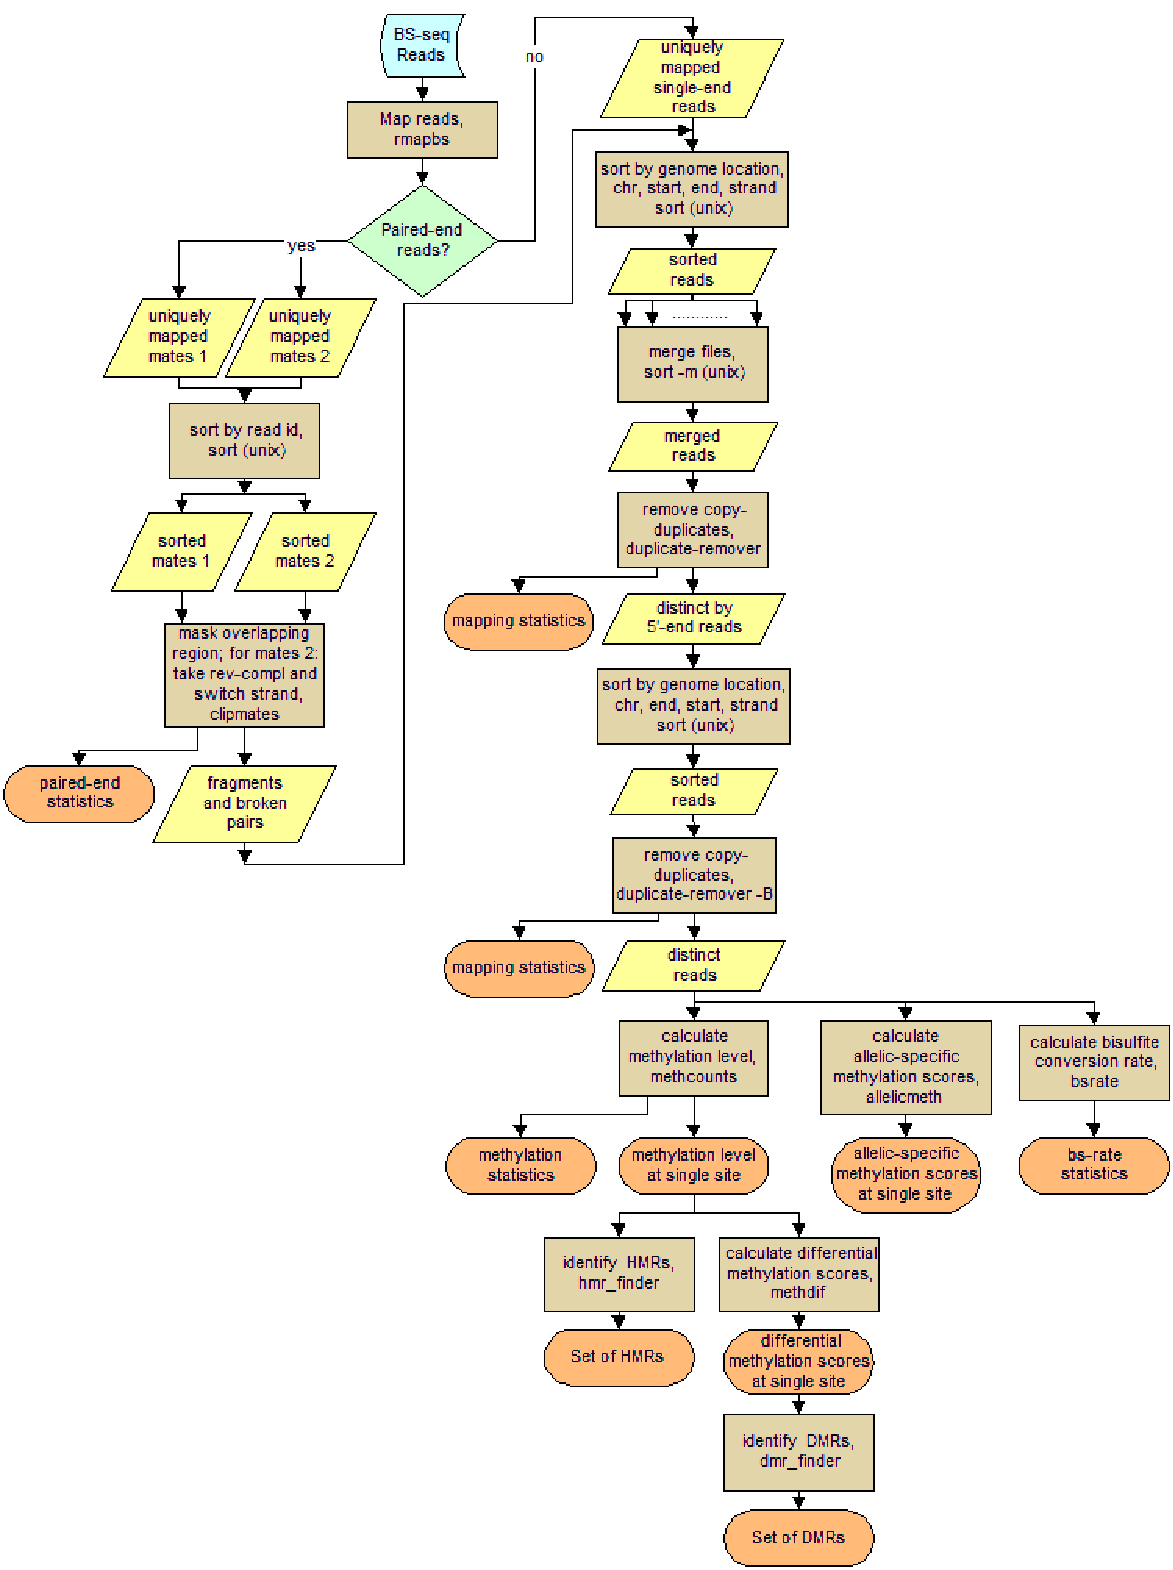
\includegraphics[width=6.3in]{figs/Methpipe_work_flow.pdf}
%   %\caption{Methpipe's Workflow}
%   %\label{fig:workflow}
% %\end{figure}

% Example data, consiting of BS-seq data from human (?) embryonic stem
% cells (ESC) and normal human foreskin fibroblasts (NHFF), has been
% provided as a tool for learning how to use the pipeline. We will refer
% to this data in the examples that illustrate each step of the pipeline
% and feel that the consistency and continuity afforded by such an
% approach will provide for the clearest learning experience. The ESC
% data consists of paired-end reads while the NHFF data consists of
% single\_end reads.

% \textbf{NOTE: I changed these file names. If these file actually
% exist, their names should be correspondingly changed.}\\

% The following are the three file names of the provided example
% data. These files are in FASTQ format, the format you should make sure
% your BS-seq data are in before running Methpipe on them. Two files
% belong to the ESC data set, where a "\_1" denontes the 5' end reads
% and a "\_2" denotes the 3' end reads (one file for each paired-end
% read type). The third file contains all of the single end reads of the
% NHFF data set.
% \begin{verbatim}
% Human_ESC_1.fastq, Human_ESC_2.fastq, Human_NHFF.fastq
% \end{verbatim}
% An example reference genome, to which both cell types map, is located
% in the directory \fn{hg18}. This genome is broken into 24 separate
% files (1 per chromsome), each named as \fn{chr*.fa} where \fn{*}
% denotes the chromosome number (or 'X' or 'Y' for the sex chromosomes).
% For each component of the pipeline, we complement discussion of the
% theory and purpose of each step by highlighting program options and
% input/output formats. For each of the two cell types, and example
% command will be shown for each step of Methpipe. This example command
% will only contain the basic options that are neccessary for the
% command to run.

% \section{Post-mapping processing}
% \label{sec:postmapping}

% Before mapped reads can be processed for higher level analyses,
% certain error avoiding steps must be taken. Paired mates can have
% overlapping regions, A-rich reads must be converted to T-rich reads
% through reverse complemetation, and read duplicates that are likely to
% be by-products of PCR overamplication must be excluded. The following
% sections discuss how to address each of these using Methpipe.

\subsection{Computing average methylation level in a genomic interval}
\label{sec:roimethstat}

One of the most common analysis tasks is to compute the average
methylation level through a genomic region. The \prog{roimethstat}
program accomplishes this. It takes a sorted \prog{methcounts} output
file and a sorted BED format file of genomic ``regions of interest''
(hence the ``roi'' in \prog{roimethstat}).  If either file is not
sorted by (chrom,end,start,strand) it can be sorted using the
following command:
\begin{verbatim}
$ LC_ALL=C sort -k 1,1 -k 3,3g -k 2,2g -k 6,6 \
         -o regions_ESC_Meth.bed.sorted regions_ESC_Meth.bed
\end{verbatim}
From there, \prog{roimethstat} can be run as follows:
\begin{verbatim}
$ ./roimethstat -o regions_ESC_Meth.bed regions.bed Human_ESC_Meth.bed.sorted
\end{verbatim}
The output format is also 6-column BED, and the score column now takes
the average methylation level through the interval, weighted according
to the number of reads informing about each CpG or C in the
methylation file. The 4th, or "name" column encodes several other
pieces of information that can be used to filter the regions. The
original name of the region in the input regions file is retained, but
separated by a colon (\lit{:}) are, in the following order, (1) the
number of CpGs in the region, (2) the number of CpGs covered at least
once, (3) the number of observations in reads indicating in the region
that indicate methylation, and (4) the total number of observations
from reads in the region. The methylation level is then (3) divided by
(4). Example output might look like:
\begin{verbatim}
chr1  3011124  3015902  REGION_A:18:18:105:166  0.63253  +
chr1  3015904  3016852  REGION_B:5:5:14:31  0.451613  +
chr1  3017204  3017572  REGION_C:2:2:2:9  0.222222  -
chr1  3021791  3025633  REGION_D:10:10:48:73  0.657534  -
chr1  3026050  3027589  REGION_E:2:4:4:32:37  0.864865  -
\end{verbatim}
Clearly if there are no reads mapping in a region, then the
methylation level will be undefined. By default \prog{roimethstat}
does not output such regions, but sometimes they are helpful, and
using the \op{-P} flag will force \prog{roimethstat} to print these
lines in the output (in which case every line in the input regions
will have a corresponding line in the output).

% Example1: ./roimethstat -v -P -o methStats.bed -r regionInterest.bed methFile.bed
% Example2: ./roimethstat -r regionInterest.bed -v -o methStats.bed methFile.bed -P
% Typical Run: ./roimethstat -v methFile.bed -r regionInterest.bed -o methStats.bed

% The output file will also be bed-formatted.  It will be in the
% following format:

% chr#    GenoStart    GenoEnd        name:cpgs:cpgs_with_reads:meth:reads    frac_cpgs_meth    Strand

% The fourth column contains the following information:

% 1) The name of each region
% 2) The number of CpGs in each region
% 3) The number of these CpGs that have at least 1 read
% 4) The total number of methylation counts in this region
% 5) The total number of reads in this region

% To seperate the ':' delimited data into tab delimited data you can
% use one of the following two commands:

% 1) sed 's/:/\t/g' [filename]
% 2) cat [filename] | tr ':' '\t'

\section{Creating UCSC Genome Browser tracks}
\label{sec:browser}

To view the methylation level or read coverage at individual CpG sites
in a genome browser, one needs to create a \lit{bigWig} format file
from a \fn{*\_Meth.bed} file, which is the output of \prog{methcount}
program. A methcount file would look like this:
\begin{verbatim}
chr1	468	469	CpG:30	0.7	+
chr1	470	471	CpG:29	0.931034	+
chr1	483	484	CpG:36	0.916667	+
chr1	488	489	CpG:36	1	+
\end{verbatim}
The first 3 columns shows the physical location of each CpG sites in
the reference genome. The number in the 4th column indicates the
coverage at each CpG site. The methylation level at individual CpG
sites can be found in the 5th column. To create methylation level
tracks or read coverage tracks, one can follow these steps:
\begin{enumerate}
\item Download the \prog{wigToBigWig} program from UCSC genome
  browser's directory of binary utilities
  (\url{http://hgdownload.cse.ucsc.edu/admin/exe/}).
\item Use the \fn{fetchChromSizes} script from the same directory to
  create the \fn{*.chrom.sizes} file for the UCSC database you are
  working with (e.g. hg18). Note that this is the file that is
  referred to as \fn{hg18.chrom.sizes} in step 3.
\item To create a \fn{bw} track for methylation level at single CpG
  sites, modify and use the following command:
\begin{verbatim}
$ cut -f 1-3,5 Human_ESC_Meth.bed | \
     wigToBigWig /dev/stdin hg18.chrom.sizes Human_ESC_Meth.bw
\end{verbatim}
  To create a \fn{bw} track for coverage at single CpG sites, modify
  and use the following command:
\begin{verbatim}
$ tr ':' '[Ctrl+v Tab]' < Human_ESC_Meth.bed | cut -f 1-3,5 | \
     wigToBigWig /dev/stdin hg18.chrom.sizes Human_ESC_Reads.bw
\end{verbatim}
\end{enumerate}
Note that if the \prog{wigToBigWig} or \prog{fetchChromSizes} programs
are not executable when downloaded, do the following:
\begin{verbatim}
$ chmod +x wigToBigWig
$ chmod +x fetchChromSizes
\end{verbatim}

\noindent
You might also want to create \fn{bigBed} browser tracks for HMRs,
AMRs or DMRs. To do so, follow these steps:
\begin{enumerate}
\item Download the \prog{bedToBigBed} program from the UCSC Genome
  Browser directory of binary utilities
  (\url{http://hgdownload.cse.ucsc.edu/admin/exe/}).
\item Use the \fn{fetchChromSizes} script from the same directory to
  create the \fn{*.chrom.sizes} file for the UCSC database you are
  working with (e.g. hg18). Note that this is the file that is
  referred to as \fn{hg18.chrom.sizes} in step 3.
\item Modify and use the following commands: For \fn{*\_HMR.bed} files
  with non-integer score in their 5th column, one needs to round the
  score to integer value, for example:
\begin{verbatim}
$ awk -v OFS="\t" '{print $1,$2,$3,$4,int($5)}' Human_ESC_HMR.bed | \
         bedToBigBed /dev/stdin hg18.chrom.sizes Human_ESC_HMR.bb
\end{verbatim}
  In the above command, since the HMRs are not stranded, we do not
  print the 6th column. Keeping the 6th column would make all the HMRs
  appear as though they have a direction -- but it would all be the
  \lit{+} strand.
\begin{verbatim}
$ bedToBigBed Human_ESC_HMR.bed hg18.chrom.sizes Human_ESC_HMR.bb
\end{verbatim}
\end{enumerate}

\subsection{Creating custom tracks for direct upload}

If you do not have access to a web server on which to provide BigBed
or BigWig files, you can still create tracks to display methylation
levels. Note that in this case the tracks will be huge and must be
transferred in their entirety to the remote UCSC Genome
Browser. Likely this is not an optimal way to be visualizing data.  To
create a track for methylation level at single CpG sites:
\begin{verbatim}
$ cut -f 1-3,5 Human_ESC_Meth.bed > Human_ESC_Meth.bedGraph
$ gzip Human_ESC_Meth.bedGraph
\end{verbatim}
To create a track for coverage at single CpG sites:
\begin{verbatim}
$ tr ':' '[Ctrl+v TAB]' < Human_ESC_Meth.bed | \
         cut -f 1-3,5 > Human_ESC_Reads.bedGraph
$ gzip Human_ESC_CpG_Reads.bedGraph
\end{verbatim}
Note that hitting \lit{Ctrl+v} then hitting \lit{TAB} produces the tab
character in a terminal window -- not needed when passing this as a
delimiter to \prog{awk}. These files can be directly uploaded to the
browser. If track headers are desired, they can be included in the
\fn{.bedGraph} files before using \prog{gzip}.  {\em Need a concise
  way here to produce tracks for all Cs, not just CpGs.}

% As for a track for methylation level at all Cs:
% \begin{verbatim}
% $ grep - Human_ESC_Cs_methcounts.bed | awk '{print $1"\t"$2"\t"$3"\t"$5*-1}' > temp3;
% $ grep + Human_ESC_Cs_methcounts.bed | awk '{print $1"\t"$2"\t"$3"\t"$5}' > temp4;
% $ cat temp3 temp4 | sort | sed -e "1i\\track type="bedGraph" name="Human_ESC_Cs_methcounts" \
% color=0,128,0 visiblity=full" > Human_ESC_Cs_methcounts.bedGraph> ;
% rm temp3 temp4
% gzip Human_ESC_Cs_methcounts.bedGraph
% \end{verbatim}

\bibliographystyle{plain}
\bibliography{biblio}

\end{document}
